\documentclass[12pt,a4paper]{article}
\usepackage[utf8]{inputenc}
\usepackage[french]{babel}
\usepackage[T1]{fontenc}
\usepackage{geometry}
\geometry{top=2.5cm, bottom=2.5cm, left=2.5cm, right=2.5cm}
\usepackage{graphicx}
\usepackage{hyperref}
\usepackage{listings}
\usepackage{xcolor}
\usepackage{fancyhdr}
\usepackage{amsmath}
\usepackage{titlesec}
\usepackage{booktabs}
\usepackage{lmodern}

% Hyperref setup
\hypersetup{
    colorlinks=true,
    linkcolor=purple,
    filecolor=magenta,      
    urlcolor=blue,
    pdftitle={Rapport de Projet - Plateforme Multi-Rôles de Gestion des Absences},
}

% Colors setup matching the Glassmorphism theme
\definecolor{accentpurple}{RGB}{139, 92, 246}
\definecolor{accentblue}{RGB}{59, 130, 246}
\definecolor{bgdark}{RGB}{11, 15, 25}
\definecolor{codegray}{rgb}{0.96,0.96,0.96}
\definecolor{codecomment}{rgb}{0.25,0.6,0.25}
\definecolor{keywordcolor}{rgb}{0.7,0.1,0.5}

% Listings setup for code blocks
\lstset{
    backgroundcolor=\color{codegray},
    commentstyle=\color{codecomment},
    keywordstyle=\color{keywordcolor}\bfseries,
    numberstyle=\tiny\color{gray},
    stringstyle=\color{accentblue},
    basicstyle=\ttfamily\small,
    breakatwhitespace=false,         
    breaklines=true,                 
    captionpos=b,                    
    keepspaces=true,                 
    numbers=left,                    
    numbersep=5pt,                  
    showspaces=false,                
    showstringspaces=false,
    showtabs=false,                  
    tabsize=4,
    language=Java
}

% Header and Footer setup
\pagestyle{fancy}
\fancyhf{}
\lhead{\footnotesize Plateforme Multi-Rôles de Gestion des Absences}
\rhead{\footnotesize Rapport de Projet - DDSIG1}
\cfoot{\thepage}

\begin{document}

% ==========================================
% PAGE DE GARDE (TITLE PAGE)
% ==========================================
\begin{titlepage}
    \centering
    \vspace*{1.0cm}
    
    {\scshape\LARGE École Marocaine des Sciences de l'Ingénieur (EMSI)} \\
    \vspace{0.4cm}
    {\scshape\large Filière : DDSIG1} \\
    
    \vspace{1.5cm}
    \rule{\linewidth}{0.8mm} \\
    \vspace{0.4cm}
    {\huge\bfseries RAPPORT DE PROJET ACADÉMIQUE DÉTAILLÉ \\}
    \vspace{0.4cm}
    {\Large\bfseries Plateforme de Gestion des Absences Multi-Rôles \\}
    \vspace{0.3cm}
    {\large Spécifications Fonctionnelles V2, Architecture JPA, Sessions \& Cookies} \\
    \rule{\linewidth}{0.8mm} \\
    
    \vspace{1.5cm}
    
    \begin{minipage}{0.48\textwidth}
        \begin{flushleft} \large
            \emph{Membres d'équipe :}\\
            \vspace{0.2cm}
            \textbf{Nizar Belkhadir} \\
            \textbf{Adam Bibilou} \\
            \textbf{Adam Asaas} \\
            \textbf{Chafiq Mwiyeh}
        \end{flushleft}
    \end{minipage}
    \hfill
    \begin{minipage}{0.48\textwidth}
        \begin{flushright} \large
            \emph{Présenté devant :} \\
            \vspace{0.2cm}
            \textbf{Pr. Houssam BAZZA} \\
            \vspace{0.4cm}
            \emph{Module :} \\
            \textbf{JEE et Génie Logiciel}
        \end{flushright}
    \end{minipage}
    
    \vfill
    \rule{8cm}{0.2mm} \\
    \vspace{0.2cm}
    {\large Année Universitaire : 2025/2026}
\end{titlepage}

\newpage
\tableofcontents
\newpage

% ==========================================
% SECTION 1
% ==========================================
\section{Introduction et Contexte du Projet}

\subsection{Problématique de l'assiduité universitaire}
Dans le cadre de la gestion académique au sein des établissements d'enseignement supérieur, le suivi de l'assiduité des étudiants représente un facteur déterminant pour garantir la rigueur pédagogique et lutter contre le décrochage scolaire. La saisie manuelle des absences, l'archivage physique des justificatifs médicaux et le calcul fastidieux des statistiques d'assiduité sont des tâches chronophages pour le corps administratif.

Un système défaillant ou obsolète engendre de nombreux problèmes :
\begin{itemize}
    \item \textbf{Perte d'informations :} Perte de justificatifs papier déposés auprès de l'administration.
    \item \textbf{Erreurs de saisie :} Incohérences lors du report manuel des absences saisies par les enseignants.
    \item \textbf{Manque de réactivité :} Les étudiants ne sont informés de leurs absences qu'en fin de semestre, rendant impossible toute contestation rapide ou rattrapage.
\end{itemize}

Ce projet vise à relever ces défis en concevant une plateforme interactive multi-rôles permettant d'interconnecter directement l'administration scolaire, les professeurs et les étudiants, assurant un traitement transparent et collaboratif de l'assiduité.

\subsection{Choix Technologique : Java EE 8 pur et JPA}
Afin d'acquérir une compréhension profonde des mécanismes internes des architectures logicielles d'entreprise, nous avons opté pour le développement d'une application en \textbf{Java EE 8 pur (Jakarta EE 8)} sans recours aux frameworks d'auto-configuration de type Spring Boot. Cette approche permet de manipuler directement :
\begin{itemize}
    \item Les cycles de vie des \textbf{Servlets} HTTP.
    \item Le rendu dynamique par \textbf{JSP} (JavaServer Pages) avec Expression Language (EL) et JSTL.
    \item La gestion de persistance par \textbf{JPA} (fournisseur Hibernate) avec requêtes JPQL.
    \item La conteneurisation de la base de données relationnelle via \textbf{PostgreSQL 15} sous Docker.
\end{itemize}

% ==========================================
% SECTION 2 : METHODOLOGIE SCRUM
% ==========================================
\section{Méthodologie de Gestion de Projet (Scrum)}
Dans le cadre de la planification et de l'exécution de notre plateforme, nous avons adopté la méthodologie agile \textbf{Scrum}. Ce cadre de travail nous a permis de structurer nos développements en cycles cours, de réagir rapidement aux contraintes techniques et de garantir un incrément logiciel de haute qualité.

\subsection{Composition de l'Équipe Scrum}
L'équipe est composée des rôles agiles suivants :
\begin{itemize}
    \item \textbf{Product Owner (PO) :} Représente les besoins de l'administration scolaire et du corps enseignant (EMSI). Il est responsable de la spécification et de la priorisation des exigences (User Stories).
    \item \textbf{Scrum Master (SM) :} \textbf{Nizar Belkhadir} — Assure la bonne application des pratiques Scrum, anime les rituels agiles, résout les blocages techniques (Git, Docker, etc.) et maintient la vélocité de l'équipe.
    \item \textbf{Équipe de Développement (Development Team) :} \textbf{Nizar, Adam B., Adam A., Chafiq}. Équipe pluridisciplinaire responsable de la conception UML, du développement des composants front-end (JSP, CSS), back-end (Servlets, DAOs) et du déploiement.
\end{itemize}

\subsection{Découpage et Objectifs des Sprints}
Le projet a été développé sur une durée globale de trois semaines, découpée en trois Sprints successifs d'une semaine chacun :
\begin{enumerate}
    \item \textbf{Sprint 1 : Conception, Persistance et Charte Graphique} \\
    Ce premier sprint a permis d'analyser le besoin et de concevoir les diagrammes UML (Cas d'utilisation, Classes, Séquence). Nous avons initialisé le projet Maven, configuré la base de données PostgreSQL 15 sous Docker et mappé les entités JPA persistantes (\texttt{Etudiant}, \texttt{Absence}, etc.). Nous avons également mis en place l'architecture de persistance isolée (\texttt{JPAUtil} et \texttt{ThreadLocal}) et créé la charte graphique moderne en CSS.
    \item \textbf{Sprint 2 : Cœur Applicatif et Sécurité des Accès} \\
    L'objectif de ce sprint était d'implémenter le moteur de traitement. Nous avons écrit la Servlet unique de routage (\texttt{AbsenceServlet}) appliquant le patron Front Controller, géré les sessions utilisateurs (\texttt{HttpSession}), et conçu la feuille d'appel interactive avec enregistrement groupé pour les professeurs, ainsi que le registre global d'administration et l'export CSV.
    \item \textbf{Sprint 3 : Workflows de Modération, Tests et Polissage} \\
    Durant le dernier sprint, nous avons développé le dashboard étudiant et ses statistiques d'assiduité, les workflows d'upload de justificatifs médicaux, et les réclamations. Nous avons configuré la mémorisation de connexion par Cookies « Remember Me » et le filtrage client en Vanilla JS. Ce sprint s'est achevé par la mise en place de la suite de tests unitaires sous \textbf{JUnit 4} et la rédaction finale du rapport technique.
\end{enumerate}

\subsection{Rituels et Cérémonies Scrum}
Pour maintenir la synchronisation de l'équipe, nous avons tenu rigoureusement les cérémonies agiles suivantes :
\begin{itemize}
    \item \textbf{Sprint Planning :} Réunion hebdomadaire pour définir l'objectif du sprint et sélectionner les tâches du Backlog de produit.
    \item \textbf{Daily Stand-up :} Point quotidien de 15 minutes durant lequel chaque membre détaille ses actions de la veille, ses objectifs du jour et ses éventuels blocages.
    \item \textbf{Sprint Review :} Démo de fin de sprint devant le Product Owner pour valider la conformité de l'incrément développé.
    \item \textbf{Sprint Retrospective :} Réunion de fin de sprint pour identifier les points positifs et les axes d'amélioration.
\end{itemize}

\subsection{User Stories clés du Backlog}
\begin{table}[htbp]
    \centering
    \caption{Exemples clés de User Stories du Backlog de produit}
    \vspace{0.3cm}
    \begin{tabular}{lp{6cm}p{5cm}}
        \hline
        \textbf{Rôle} & \textbf{User Story} & \textbf{Objectif Métier} \\
        \hline
        Professeur & En tant qu'enseignant, je veux faire l'appel sur une grille interactive & Enregistrer les absences rapidement. \\
        Étudiant & En tant qu'étudiant, je veux téléverser un certificat médical PDF & Justifier mes absences auprès de l'administration. \\
        Administrateur & En tant qu'administrateur, je veux exporter les absences en CSV & Analyser et éditer les données sous Microsoft Excel. \\
        Étudiant & En tant qu'étudiant, je veux contester une absence indue & Permettre sa suppression par l'administrateur. \\
        \hline
    \end{tabular}
\end{table}

% ==========================================
% SECTION 3
% ==========================================
\section{Cahier des Charges et Spécifications Fonctionnelles}

\subsection{Description des Rôles Applicatifs}
L'architecture de l'application s'articule autour de trois rôles distincts, chacun disposant d'un espace applicatif sécurisé :

\subsubsection{Espace Administration (Admin)}
L'administrateur scolaire est le garant de la cohérence globale du système. Ses droits comprennent :
\begin{itemize}
    \item Consultation du registre global de toutes les absences déclarées.
    \item Saisie manuelle d'une absence (par exemple, pour régulariser des séances particulières).
    \item Modération des demandes de justificatifs d'absence soumises par les étudiants.
    \item Modération des demandes de réclamation soumises par les étudiants.
    \item Exportation de l'historique complet des absences au format CSV pour Excel.
\end{itemize}

\subsubsection{Espace Enseignant (Professeur)}
L'enseignant est chargé de l'appel pour les cours qui lui sont attribués :
\begin{itemize}
    \item Accès à la liste de ses cours et séances d'enseignement.
    \item Saisie rapide et interactive de la feuille d'appel pour une séance spécifique.
    \item Ajout automatique des absences pour les étudiants cochés absents, et suppression automatique si un étudiant est décoché.
\end{itemize}

\subsubsection{Espace Étudiant}
L'étudiant dispose d'un accès en lecture à ses propres données et peut formuler des demandes d'ajustement :
\begin{itemize}
    \item Visualisation de ses statistiques personnelles (nombre total d'absences, absences justifiées, absences injustifiées).
    \item Dépôt d'une demande de justification (renseignant un motif textuel et une pièce justificative PDF/image optionnelle).
    \item Dépôt d'une réclamation pour signaler qu'il a été noté absent par erreur lors d'un cours où il était présent.
\end{itemize}

\subsection{Cycle de Vie des Demandes de Régularisation}
Pour assurer la modération sans supprimer les données arbitrairement, nous avons modélisé deux workflows distincts :
\begin{itemize}
    \item \textbf{Flux de Justification :} L'étudiant soumet un motif et un fichier. L'absence passe au statut de justification \texttt{PENDING}. L'administrateur examine la demande : s'il l'accepte, le statut devient \texttt{ACCEPTED} et l'absence est considérée comme justifiée. S'il la refuse, le statut devient \texttt{REJECTED} et l'absence reste injustifiée.
    \item \textbf{Flux de Réclamation :} L'étudiant déclare sa présence indue. L'absence passe au statut de réclamation \texttt{PENDING}. L'administrateur valide : s'il accepte la réclamation, l'absence est supprimée de la base de données. S'il la rejette, le statut devient \texttt{REJECTED} et l'absence est maintenue.
\end{itemize}

\section{Partie Conception (Modélisation UML)}

\subsection{Diagramme de Cas d'Utilisation (Use Case Diagram)}
Le diagramme de cas d'utilisation synthétise les limites fonctionnelles du système et définit les rôles d'accès de chaque acteur (Étudiant, Professeur, Administrateur). Il permet d'illustrer visuellement les cas d'utilisation clés tels que la saisie d'absence, le dépôt de justificatif, et l'arbitrage des réclamations.

\begin{figure}[htbp]
    \centering
    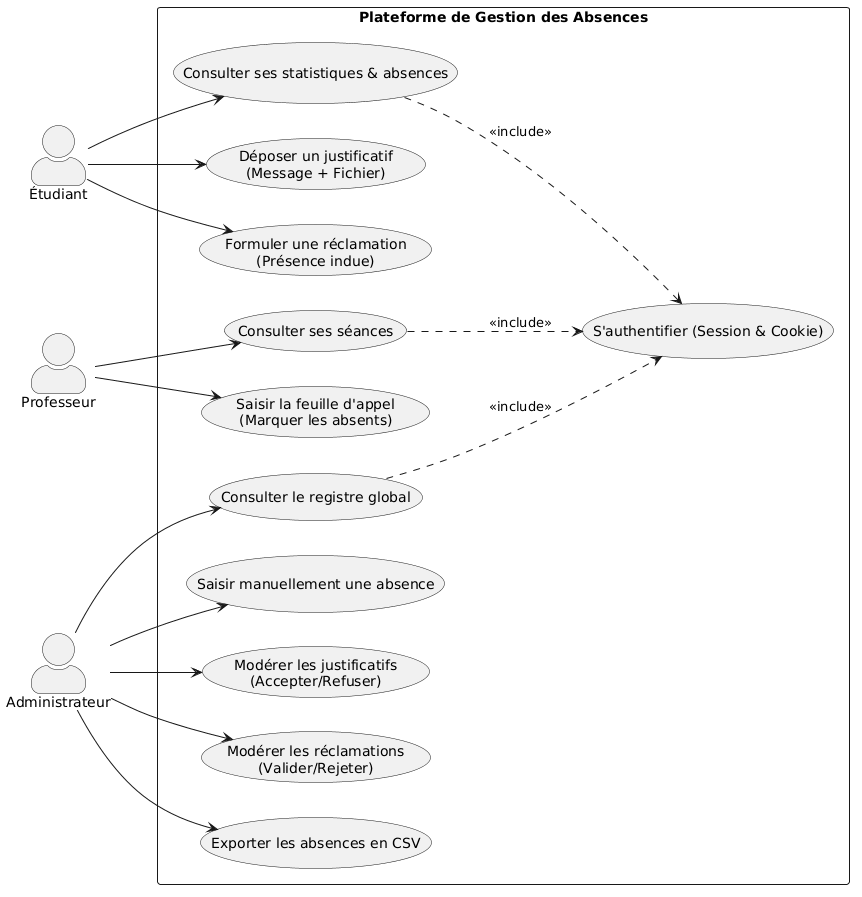
\includegraphics[width=0.8\textwidth]{use_case.png}
    \caption{Diagramme de Cas d'Utilisation - Plateforme de Gestion des Absences}
    \label{fig:use_case}
\end{figure}

\subsection{Diagramme de Classes (Class Diagram)}
Le diagramme de classes représente le modèle conceptuel de données de notre domaine d'application. Chaque classe est directement mappée en entité JPA. Les relations modélisent l'association d'un étudiant à ses absences, d'une absence à une séance de cours spécifique, et d'un cours à un enseignant responsable.

\begin{figure}[htbp]
    \centering
    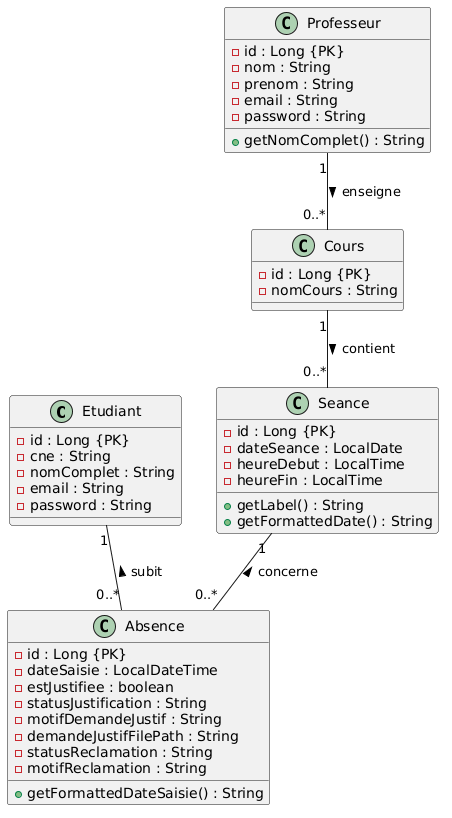
\includegraphics[width=0.8\textwidth]{class_diagram.png}
    \caption{Diagramme de Classes JPA - Modèle du Domaine}
    \label{fig:class_diagram}
\end{figure}

\subsection{Diagramme de Séquence (Sequence Diagram)}
Le diagramme de séquence retrace les interactions temporelles entre les composants du système (Client JSP, Contrôleur Servlet, DAOs et Base de données PostgreSQL) lors d'un scénario type de soumission et de validation d'un justificatif d'absence.

\begin{figure}[htbp]
    \centering
    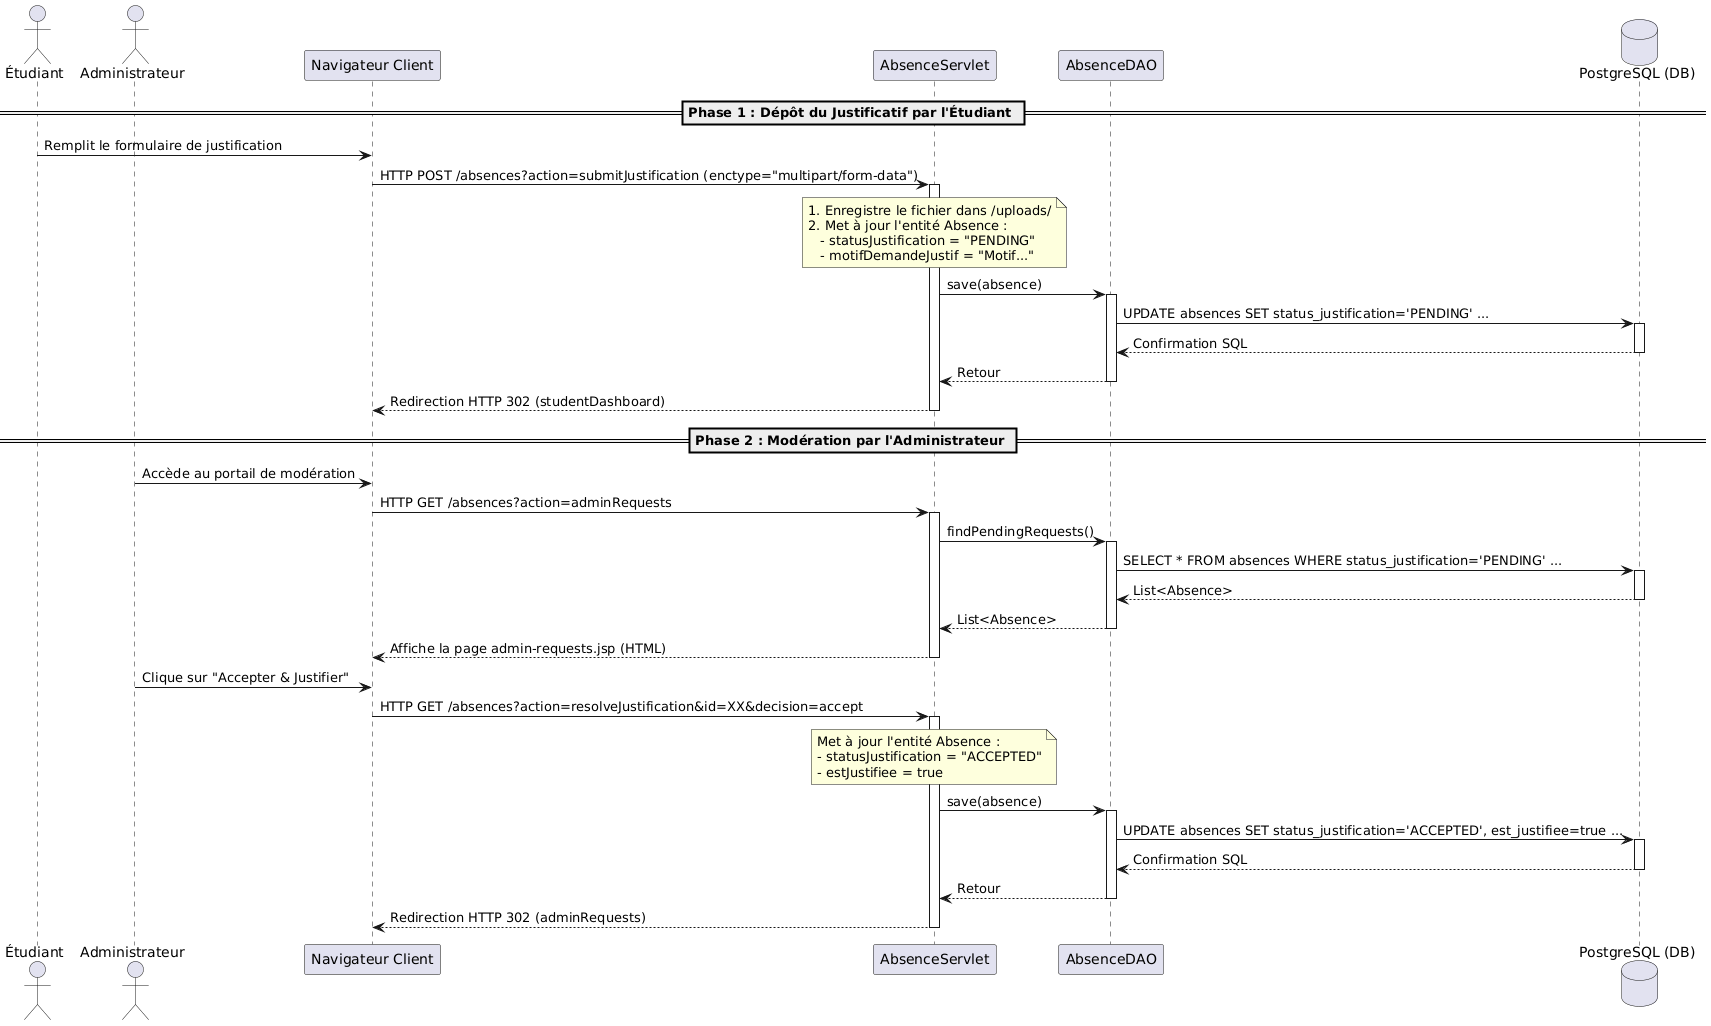
\includegraphics[width=0.8\textwidth]{sequence_diagram.png}
    \caption{Diagramme de Séquence - Traitement des Demandes et Persistance}
    \label{fig:sequence_diagram}
\end{figure}

% ==========================================
% SECTION 4
% ==========================================
\section{Patrons de Conception (Design Patterns) Appliqués}
Afin de concevoir une application modulaire, extensible et conforme aux bonnes pratiques du Génie Logiciel, plusieurs patrons de conception (\textit{Design Patterns}) ont été implémentés au sein de l'architecture de la plateforme.

\subsection{Modèle-Vue-Contrôleur (MVC)}
Le patron de conception architectural central est le \textbf{MVC}. Il sépare l'application en trois composants indépendants :
\begin{itemize}
    \item \textbf{Le Modèle (Model) :} Représenté par les entités JPA (\texttt{Etudiant}, \texttt{Absence}, \texttt{Professeur}, \texttt{Seance}, \texttt{Cours}) et la couche de persistance. Il gère l'état et l'accès aux données de manière isolée.
    \item \textbf{La Vue (View) :} Représentée par les pages JSP sous \texttt{WEB-INF/views/}. Elles s'occupent uniquement du rendu graphique de l'interface et du dynamisme d'affichage via JSTL et EL, sans contenir de logique métier.
    \item \textbf{Le Contrôleur (Controller) :} Représenté par la servlet \texttt{AbsenceServlet} qui intercepte les requêtes HTTP, sollicite le modèle et sélectionne la vue appropriée.
\end{itemize}

\subsection{Front Controller (Contrôleur Frontal)}
Plutôt que d'associer un servlet distinct à chaque URL (ce qui alourdirait la maintenance et fragmenterait la gestion de la sécurité), la plateforme implémente le pattern \textbf{Front Controller}. Une servlet unique (\texttt{AbsenceServlet}) intercepte toutes les requêtes mappées sous \texttt{/absences}. Elle réalise les vérifications de session transversales (Session Gating) et de rôles, puis aiguille le traitement vers la méthode dédiée en fonction du paramètre \texttt{action} passé en paramètre d'URL.

\subsection{Data Access Object (DAO)}
Le pattern \textbf{DAO} isole complètement la logique d'accès à la base de données relationnelle du reste de l'application. La servlet contrôleur n'effectue jamais de requêtes JPQL en direct. Elle délègue ces opérations à des classes spécialisées (\texttt{AbsenceDAO}, \texttt{EtudiantDAO}, etc.). Cela permet de découpler le modèle physique de stockage de la logique applicative.

\subsection{Singleton (Unique Instance)}
La fabrique d'EntityManager (\texttt{EntityManagerFactory}) est une ressource lourde à initialiser. Nous appliquons le principe du \textbf{Singleton} encapsulé dans la classe \texttt{JPAUtil}. L'EntityManagerFactory est instancié une seule fois lors du démarrage du conteneur Tomcat par le listener \texttt{JPAInitializer} et partagé sous forme d'instance unique tout au long du cycle de vie de l'application.

\subsection{ThreadLocal Context (Isolation par Thread)}
Puisque l'\texttt{EntityManager} standard de JPA n'est pas thread-safe, son partage direct entre requêtes HTTP concurrentes corromprait la session de persistance. Nous utilisons le pattern \textbf{ThreadLocal} dans \texttt{JPAUtil} pour lier chaque instance d'EntityManager au thread courant exécutant la requête HTTP. Chaque appelant dispose ainsi d'un gestionnaire de persistance isolé et sécurisé, détruit en fin de cycle de requête.

\newpage

% ==========================================
% SECTION 4
% ==========================================
\section{Infrastructure, Persistance et Couche Modèle}

\subsection{Conteneurisation Database (PostgreSQL et Docker)}
La base de données PostgreSQL est configurée via un fichier Docker Compose facilitant le déploiement sur le port physique local \texttt{5436}.

\begin{lstlisting}[language=XML, caption={Fichier docker-compose.yml}]
version: '3.8'
services:
  db:
    image: postgres:15
    container_name: postgres_jee_absences
    environment:
      POSTGRES_DB: gestion_absences
      POSTGRES_USER: postgres
      POSTGRES_PASSWORD: postgres
    ports:
      - "5436:5432"
    volumes:
      - pgdata:/var/lib/postgresql/data

volumes:
  pgdata:
\end{lstlisting}

\subsection{Configuration de JPA (\texttt{persistence.xml})}
L'unité de persistance JPA configure le driver PostgreSQL JDBC et la génération automatique du schéma de tables.

\begin{lstlisting}[language=XML, caption={Fichier persistence.xml}]
<persistence xmlns="http://xmlns.jcp.org/xml/ns/persistence" version="2.1">
    <persistence-unit name="AbsencePU" transaction-type="RESOURCE_LOCAL">
        <provider>org.hibernate.jpa.HibernatePersistenceProvider</provider>
        <class>com.gestionabsences.model.Etudiant</class>
        <class>com.gestionabsences.model.Cours</class>
        <class>com.gestionabsences.model.Seance</class>
        <class>com.gestionabsences.model.Absence</class>
        <class>com.gestionabsences.model.Professeur</class>
        <properties>
            <property name="javax.persistence.jdbc.driver" value="org.postgresql.Driver" />
            <property name="javax.persistence.jdbc.url" value="jdbc:postgresql://localhost:5436/gestion_absences" />
            <property name="javax.persistence.jdbc.user" value="postgres" />
            <property name="javax.persistence.jdbc.password" value="postgres" />
            
            <property name="hibernate.dialect" value="org.hibernate.dialect.PostgreSQL95Dialect" />
            <property name="hibernate.hbm2ddl.auto" value="update" />
            <property name="hibernate.show_sql" value="true" />
            <property name="hibernate.format_sql" value="true" />
        </properties>
    </persistence-unit>
</persistence>
\end{lstlisting}

\subsection{Implémentation des Classes du Domaine (Modèles JPA)}
Dans le cadre de l'architecture JPA, chaque table de la base de données PostgreSQL est représentée par une classe Java annotée (Entity). Afin d'assurer une séparation propre des préoccupations (Clean Architecture), ces entités se concentrent sur le mapping relationnel.

Voici la description conceptuelle de nos cinq entités principales :
\begin{enumerate}
    \item \textbf{Etudiant :} Modélise un étudiant identifié de manière unique par son CNE. Il possède des attributs de connexion (email et mot de passe) et son nom complet.
    \item \textbf{Professeur :} Représente l'enseignant responsable des appels. Il possède un nom, prénom, email et mot de passe.
    \item \textbf{Cours :} Représente une matière enseignée, associée à un professeur unique via une relation de type plusieurs-à-un (\texttt{ManyToOne}).
    \item \textbf{Seance :} Représente un créneau horaire de cours (date, heure de début, heure de fin) rattaché à un cours.
    \item \textbf{Absence :} C'est l'entité centrale du système. Elle lie un étudiant à une séance de cours spécifique et porte les statuts de justification et de réclamation.
\end{enumerate}

Pour illustrer le paramétrage JPA de notre projet, nous présentons ci-dessous un extrait de la classe \texttt{Absence.java} montrant la configuration des clés étrangères, de la contrainte d'unicité (un étudiant ne peut avoir qu'une seule absence par séance) et des nouveaux champs de modération :

\begin{lstlisting}[caption={Extrait JPA de la classe Absence.java}]
@Entity
@Table(name = "absences", uniqueConstraints = {
    @UniqueConstraint(columnNames = {"etudiant_id", "seance_id"})
})
public class Absence implements Serializable {
    @Id
    @GeneratedValue(strategy = GenerationType.IDENTITY)
    private Long id;

    @ManyToOne(fetch = FetchType.EAGER)
    @JoinColumn(name = "etudiant_id", nullable = false)
    private Etudiant etudiant;

    @ManyToOne(fetch = FetchType.EAGER)
    @JoinColumn(name = "seance_id", nullable = false)
    private Seance seance;

    @Column(name = "status_justification", length = 20)
    private String statusJustification = "NONE"; // NONE, PENDING, ACCEPTED, REJECTED

    @Column(name = "status_reclamation", length = 20)
    private String statusReclamation = "NONE"; // NONE, PENDING, REJECTED
}
\end{lstlisting}

% ==========================================
% SECTION 5
% ==========================================
\section{Gestion du Cycle de Vie JPA et EntityManagers}

\subsection{Le Listener de Démarrage (\texttt{JPAInitializer.java})}
Tomcat étant un conteneur de servlets léger, il n'initialise pas nativement la persistance JPA au chargement. Nous y remédions en implémentant un \texttt{ServletContextListener} annoté \texttt{@WebListener}. Ce listener instancie l'unique \texttt{EntityManagerFactory} au démarrage du serveur et le ferme proprement à l'arrêt du contexte, évitant ainsi les fuites de ressources.

\subsection{Thread Isolation des Managers (\texttt{JPAUtil.java})}
L'\texttt{EntityManager} n'étant pas thread-safe, nous utilisons la classe \texttt{ThreadLocal} de Java pour associer une instance d'EntityManager distincte à chaque thread de requête HTTP traitée par le pool de Tomcat. 

La classe utilitaire \texttt{JPAUtil} centralise cette logique, permettant à toutes les classes DAO d'obtenir de façon sécurisée le gestionnaire de persistance lié au thread courant :

\begin{lstlisting}[caption={Gestion du ThreadLocal pour l'EntityManager dans JPAUtil.java}]
public class JPAUtil {
    private static EntityManagerFactory emf;
    private static final ThreadLocal<EntityManager> threadLocalEntityManager = new ThreadLocal<>();

    public static EntityManager getEntityManager() {
        EntityManager em = threadLocalEntityManager.get();
        if (em == null || !em.isOpen()) {
            em = emf.createEntityManager();
            threadLocalEntityManager.set(em);
        }
        return em;
    }
}
\end{lstlisting}

% ==========================================
% SECTION 6
% ==========================================
\section{Couche de Persistance : Implémentation des DAOs}

\subsection{Gestion Manuelle des Transactions}
En l'absence de conteneur d'injection (comme Spring ou EJB), nous gérons manuellement le cycle de vie de chaque transaction de persistance via l'interface \texttt{EntityTransaction} du standard JPA. Les étapes respectent scrupuleusement le patron suivant :
\begin{enumerate}
    \item Récupération de l'EntityManager associé au thread courant par la méthode utilitaire \texttt{JPAUtil.getEntityManager()}.
    \item Démarrage de la transaction via \texttt{tx.begin()}.
    \item Exécution des opérations d'écriture avec \texttt{persist} ou \texttt{merge}.
    \item Validation de l'état persistant avec \texttt{tx.commit()}.
    \item En cas d'exception, annulation via \texttt{tx.rollback()} et remontée de l'erreur.
    \item Libération finale de l'EntityManager dans le bloc \texttt{finally}.
\end{enumerate}

\subsection{Le Patron Data Access Object (DAO)}
Afin de découpler la couche d'accès aux données du reste de l'application, nous avons développé trois classes DAO principales : \texttt{AbsenceDAO}, \texttt{EtudiantDAO} et \texttt{ProfesseurDAO}. Elles encapsulent les requêtes JPQL (Java Persistence Query Language) et les opérations de recherche par clé primaire.

Pour illustrer l'implémentation de nos requêtes complexes, voici un extrait de la classe \texttt{AbsenceDAO.java} montrant la récupération des requêtes en attente de modération (justifications ou réclamations) :

\begin{lstlisting}[caption={Extrait des requêtes JPQL dans AbsenceDAO.java}]
public class AbsenceDAO {
    public List<Absence> findPendingRequests() {
        EntityManager em = JPAUtil.getEntityManager();
        try {
            return em.createQuery(
                "SELECT a FROM Absence a WHERE a.statusJustification = 'PENDING' OR a.statusReclamation = 'PENDING'", 
                Absence.class
            ).getResultList();
        } finally {
            JPAUtil.closeEntityManager();
        }
    }
}
\end{lstlisting}

% ==========================================
% SECTION 7
% ==========================================
\section{Couche Contrôleur : La Servlet Front-Controller}
La Servlet centralisée \texttt{AbsenceServlet.java} gère à elle seule le cycle de routage de la plateforme, vérifiant l'authentification et dispatchant les actions.

\subsection{Vérification des Rôles et Session Gate}
Afin d'éviter tout accès illégitime, la Servlet implémente un filtre directement dans les méthodes \texttt{doGet} et \texttt{doPost} :
\begin{itemize}
    \item Extraction de la session sans création (\texttt{getSession(false)}).
    \item Si null, redirection vers le login.
    \item Si existante, comparaison de l'attribut \texttt{userRole}.
\end{itemize}

\subsection{Structure Majeure du Servlet de Contrôle}
Le servlet de contrôle centralise la logique de routage. Il analyse le paramètre \texttt{action} passé en paramètre d'URL (pattern Front-Controller) et aiguille la requête vers la méthode de traitement dédiée.

Afin d'illustrer la gestion des rôles à la connexion et le téléversement de fichiers multipart sans framework externe, voici les extraits clés de traitement :

\begin{lstlisting}[caption={Extrait de l'authentification unifiée dans AbsenceServlet.java}]
private void processLogin(HttpServletRequest request, HttpServletResponse response) 
        throws ServletException, IOException {
    String email = request.getParameter("email");
    String password = request.getParameter("password");

    // Authentification Admin
    if ("admin@univ.fr".equals(email) && "admin".equals(password)) {
        HttpSession session = request.getSession(true);
        session.setAttribute("userRole", "ADMIN");
        response.sendRedirect(request.getContextPath() + "/absences?action=list");
        return;
    }
    // Traitement des roles PROFESSEUR et ETUDIANT via les DAOs correspondants...
}
\end{lstlisting}

\begin{lstlisting}[caption={Gestion de l'upload de justificatif dans AbsenceServlet.java}]
private void processStudentJustification(HttpServletRequest request, HttpServletResponse response)
        throws ServletException, IOException {
    Long id = Long.parseLong(request.getParameter("id"));
    Part filePart = request.getPart("pieceJustificative");
    Absence abs = absenceDAO.findById(id);

    if (abs != null && filePart != null && filePart.getSize() > 0) {
        String fileName = filePart.getSubmittedFileName();
        String uniqueName = System.currentTimeMillis() + "_" + fileName;
        String uploadPath = request.getServletContext().getRealPath("") + File.separator + "uploads";
        
        filePart.write(uploadPath + File.separator + uniqueName);
        abs.setDemandeJustifFilePath("uploads/" + uniqueName);
        abs.setStatusJustification("PENDING");
        absenceDAO.save(abs);
    }
    response.sendRedirect(request.getContextPath() + "/absences?action=studentDashboard");
}
\end{lstlisting}

% ==========================================
% SECTION 8
% ==========================================
\section{Gestion d'État : Sessions \& Cookies}

\subsection{Statelessness HTTP et HttpSession}
Le protocole HTTP est par nature sans état (stateless) ; chaque requête du client est traitée de façon totalement indépendante de la précédente. Pour maintenir la continuité de l'accès au tableau de bord, la plateforme s'appuie sur la classe standard \texttt{HttpSession}.

Lorsqu'un utilisateur s'authentifie, un identifiant de session unique (\texttt{JSESSIONID}) est stocké en mémoire serveur et partagé avec le navigateur sous forme de cookie temporaire. Ce cookie est transmis à chaque requête, permettant au serveur de charger les attributs associés à la session.

\subsection{Persistance et Remplissage via Cookies}
Pour améliorer le confort d'utilisation, un Cookie persistant est créé sur le client si la case "Se souvenir de moi" est cochée.

\begin{lstlisting}[caption={Lecture des cookies au chargement du login - AbsenceServlet.java}]
private void showLoginForm(HttpServletRequest request, HttpServletResponse response)
        throws ServletException, IOException {
    Cookie[] cookies = request.getCookies();
    if (cookies != null) {
        for (Cookie c : cookies) {
            if ("rememberedAdmin".equals(c.getName())) {
                request.setAttribute("rememberedAdmin", c.getValue());
                break;
            }
        }
    }
    request.getRequestDispatcher("/WEB-INF/views/login.jsp").forward(request, response);
}
\end{lstlisting}

% ==========================================
% SECTION 9
% ==========================================
\section{Téléversement de Fichiers \& Exportations}

\subsection{Téléversement avec Multipart Config}
Pour gérer les pièces jointes des étudiants de manière sécurisée, la Servlet est configurée avec l'annotation \texttt{@MultipartConfig} qui définit des contraintes de taille sur les téléversements. Les justificatifs sont sauvés dans un dossier physique \texttt{uploads/} au sein du répertoire de déploiement web.

\subsection{Exportation CSV avec Signature BOM}
L'exportation en format CSV est codée en écrivant directement dans le flux de sortie HTTP (\texttt{response.getOutputStream()}).
Pour éviter que Microsoft Excel n'altère l'affichage des caractères accentués des noms d'étudiants (é, à, ç), nous écrivons la signature BOM UTF-8 (\texttt{0xEF, 0xBB, 0xBF}) avant d'initier l'écriture des chaînes de caractères.

% ==========================================
% SECTION 10
% ==========================================
\section{Interface Utilisateur (UI) \& CSS Glassmorphism}

\subsection{Philosophie du Design System}
Pour proposer une esthétique digne des meilleures applications Web, nous avons défini un design Glassmorphic (effet verre dépoli) basé sur des couleurs sombres, des reflets lumineux et des flous d'arrière-plan.

\begin{lstlisting}[language=HTML, caption={Design Tokens - style.css}]
:root {
    --bg-primary: #0b0f19;
    --accent-purple: #8b5cf6;
    --accent-blue: #3b82f6;
    --success: #10b981;
    --danger: #ef4444;
    --text-primary: #f8fafc;
    --glass-bg: rgba(30, 41, 59, 0.45);
    --glass-border: rgba(255, 255, 255, 0.08);
}
body {
    background-color: var(--bg-primary);
    color: var(--text-primary);
    font-family: 'Inter', sans-serif;
}
.card {
    background: var(--glass-bg);
    backdrop-filter: blur(16px);
    border: 1px solid var(--glass-border);
    border-radius: 12px;
}
\end{lstlisting}

\subsection{Filtrage client temps réel (Vanilla JS)}
Le filtrage en temps réel dans les tableaux d'absences est effectué en JavaScript côté navigateur pour une interactivité instantanée.

\begin{lstlisting}[language=HTML, caption={Filtrage interactif}]
function filterAbsences() {
    var query = document.getElementById("searchInput").value.toLowerCase();
    var filter = document.getElementById("statusFilter").value;
    var rows = document.querySelectorAll("table tbody tr");

    rows.forEach(function(row) {
        var nom = row.cells[1].textContent.toLowerCase();
        var cours = row.cells[2].textContent.toLowerCase();
        var status = row.cells[4].textContent.toLowerCase();

        var matchesQuery = nom.indexOf(query) > -1 || cours.indexOf(query) > -1;
        var matchesStatus = filter === "ALL" || 
            (filter === "JUSTIF" && status.indexOf("justifi") > -1) ||
            (filter === "NONJUSTIF" && status.indexOf("non justifi") > -1);

        row.style.display = (matchesQuery && matchesStatus) ? "" : "none";
    });
}
\end{lstlisting}

% ==========================================
% SECTION 11
% ==========================================
\section{Structure Détaillée des Vues (JSPs)}
La couche de présentation utilise des pages JSP (JavaServer Pages) associées à la bibliothèque de balises standard JSTL (JavaServer Pages Standard Tag Library). Cela permet d'éviter l'écriture de code Java brut (scriptlets) au sein des fichiers HTML, préservant ainsi le modèle MVC.

\subsection{Espace Étudiant - student-dashboard.jsp}
Cette JSP présente les statistiques de l'étudiant connecté et liste ses absences à travers un tableau interactif. L'étudiant peut initier deux processus : le dépôt de justificatif et la réclamation.

La directive JSTL ci-dessous illustre le rendu conditionnel du bouton d'action selon le statut de l'absence :

\begin{lstlisting}[language=HTML, caption={Rendu conditionnel avec JSTL dans student-dashboard.jsp}]
<c:forEach var="abs" items="${absences}">
    <tr>
        <td>${abs.formattedDateSaisie}</td>
        <td>${abs.seance.cours.nomCours}</td>
        <td>${abs.estJustifiee ? 'Justifiee' : 'Non Justifiee'}</td>
        <td>
            <c:if test="${not abs.estJustifiee}">
                <button onclick="openJustify(${abs.id})">Justifier</button>
            </c:if>
        </td>
    </tr>
</c:forEach>
\end{lstlisting}

\subsection{Espace Enseignant - prof-dashboard.jsp}
L'espace professeur implémente la feuille d'appel dynamique. L'enseignant choisit une séance, coche les étudiants absents et soumet le formulaire. La liste des étudiants est parcourue dynamiquement, et les identifiants cochés sont transmis en tableau de paramètres HTTP au servlet de contrôle :

\begin{lstlisting}[language=HTML, caption={Boucle de sélection des étudiants pour l'appel}]
<c:forEach var="st" items="${etudiants}">
    <div class="student-item">
        <span>${st.nomComplet}</span>
        <input type="checkbox" name="absentStudents" value="${st.id}">
    </div>
</c:forEach>
\end{lstlisting}

\subsection{Espace Administration - admin-requests.jsp}
Le portail de modération liste toutes les demandes reçues avec leurs motifs et les liens de téléchargement des justificatifs stockés en serveur. L'administrateur peut accepter ou rejeter chaque demande en un clic :

\begin{lstlisting}[language=HTML, caption={Actions de modération admin}]
<c:forEach var="abs" items="${pendingAbsences}">
    <div class="request-card">
        <h3>${abs.etudiant.nomComplet} - ${abs.seance.cours.nomCours}</h3>
        <p>Motif: ${abs.motifDemandeJustif}</p>
        <a href="${pageContext.request.contextPath}/absences?action=resolveJustification&id=${abs.id}&decision=accept">Accepter</a>
        <a href="${pageContext.request.contextPath}/absences?action=resolveJustification&id=${abs.id}&decision=refuse">Refuser</a>
    </div>
</c:forEach>
\end{lstlisting}

% ==========================================
% SECTION 12
% ==========================================
\section{Déploiement et Configuration}

\subsection{Configuration de déploiement (web.xml)}
Le fichier `web.xml` configure l'encodage des requêtes et le mapping d'URL racine `/absences` pour diriger le trafic vers notre Servlet de contrôle unique.

\subsection{Maven pom.xml}
Les dépendances Maven intègrent les APIs de Servlets, JSPs, JSTL, Hibernate Core et le connecteur JDBC de PostgreSQL.

% ==========================================
% SECTION 13
% ==========================================
\section{Scénarios d'Exécution et Recette de Tests}
Cette section présente la validation fonctionnelle de la plateforme à travers les différents cas d'utilisation réels et les captures d'écran associées.

\subsection{Test 1 : Authentification multi-rôle}
L'accès à l'application est sécurisé par un portail d'authentification unique aiguillant les utilisateurs selon leur rôle en base de données.
\begin{itemize}
    \item \textbf{Action :} Saisie des identifiants (administrateur, professeur ou étudiant) dans le formulaire de connexion.
    \item \textbf{Résultat attendu :} Redirection vers le dashboard correspondant.
\end{itemize}
\begin{figure}[htbp]
    \centering
    \includegraphics[width=0.85\textwidth]{uploads/test_login.jpg}
    \caption{Interface de Connexion Multi-Rôles}
    \label{fig:test_login}
\end{figure}

\subsection{Test 2 : Mémorisation de session par Cookies}
Pour améliorer l'expérience utilisateur, l'option « Se souvenir de moi » stocke un cookie sécurisé sur le client.
\begin{itemize}
    \item \textbf{Action :} Activation de la case « Se souvenir de moi » lors du login et vérification de la persistance après fermeture du navigateur.
    \item \textbf{Résultat attendu :} Création du cookie correspondant et reconnexion automatique.
\end{itemize}
\begin{figure}[htbp]
    \centering
    \includegraphics[width=0.85\textwidth]{uploads/test_cookie.jpg}
    \caption{Persistance d'authentification par Cookie HTTP}
    \label{fig:test_cookie}
\end{figure}

\subsection{Test 3 : Saisie d'appel interactif par le Professeur}
L'enseignant peut sélectionner sa séance active et réaliser l'appel rapidement.
\begin{itemize}
    \item \textbf{Action :} Sélection de la séance dans la liste déroulante, cochage des étudiants absents, et soumission.
    \item \textbf{Résultat attendu :} Création en base de données des entrées d'absences correspondantes.
\end{itemize}
\begin{figure}[htbp]
    \centering
    \includegraphics[width=0.85\textwidth]{uploads/test_prof_appel_absence.jpg}
    \caption{Feuille d'Appel Interactive de l'Enseignant}
    \label{fig:test_prof_appel}
\end{figure}

\subsection{Test 4 : Tableau de bord Étudiant et suivi personnel}
L'étudiant accède en temps réel à l'état de son assiduité et peut lancer le workflow de justification ou de réclamation.
\begin{itemize}
    \item \textbf{Action :} Consultation de la page d'accueil étudiante.
    \item \textbf{Résultat attendu :} Affichage précis du nombre total d'absences et des détails de chaque séance.
\end{itemize}
\begin{figure}[htbp]
    \centering
    \includegraphics[width=0.85\textwidth]{uploads/test_student_dashboard.jpg}
    \caption{Tableau de Bord Étudiant et Statut des Absences}
    \label{fig:test_student_db}
\end{figure}

\subsection{Test 5 : Modération administrative des justificatifs et réclamations}
L'administrateur arbitre et statue sur les demandes de régularisation déposées.
\begin{itemize}
    \item \textbf{Action :} Examen des justificatifs médicaux téléversés et clic sur « Accepter » ou « Refuser ».
    \item \textbf{Résultat attendu :} Mise à jour automatique du statut de l'absence en base de données.
\end{itemize}
\begin{figure}[htbp]
    \centering
    \includegraphics[width=0.85\textwidth]{uploads/test_admin_dmd_justification.jpg}
    \caption{Portail d'Arbitrage et de Modération Admin}
    \label{fig:test_admin_requests}
\end{figure}

\subsection{Tests Unitaires Automatisés (JUnit)}
Pour garantir la robustesse de l'application et éviter toute régression lors des phases de refactoring, nous avons intégré des tests unitaires automatisés basés sur le framework \textbf{JUnit 4}. Ces tests permettent de valider le comportement logique de nos modèles et utilitaires en isolation complète.

Trois classes de test ont été implémentées dans le répertoire \texttt{src/test/java} :
\begin{itemize}
    \item \textbf{\texttt{EtudiantTest} :} Vérifie le bon fonctionnement du constructeur, des accesseurs (Getters/Setters) et la méthode utilitaire \texttt{getNomComplet()} qui convertit automatiquement le nom de famille en majuscules.
    \item \textbf{\texttt{SeanceTest} :} Valide le formatage personnalisé de la date (\texttt{dd/MM/yyyy}) et la génération dynamique du libellé de séance combinant le nom du cours, la date et les horaires.
    \item \textbf{\texttt{JPAUtilTest} :} Teste la sécurité d'accès de la classe utilitaire de persistance en vérifiant que toute demande d'accès à l'EntityManager lève une exception \texttt{IllegalStateException} si la fabrique globale n'a pas encore été initialisée par le listener de démarrage.
\end{itemize}

\begin{lstlisting}[language=Java, caption={Extrait des tests unitaires de validation du modèle Etudiant}]
package com.gestionabsences;

import com.gestionabsences.model.Etudiant;
import org.junit.Test;
import static org.junit.Assert.*;

public class EtudiantTest {
    @Test
    public void testGetNomComplet() {
        Etudiant etudiant = new Etudiant("CNE999", "belkhadir", "nizar", "nizar@univ.fr");
        assertEquals("BELKHADIR nizar", etudiant.getNomComplet());
    }
}
\end{lstlisting}

% ==========================================
% SECTION 14
% ==========================================
\section{Conclusion et Perspectives}
L'architecture robuste de cette plateforme multi-rôles en Java EE 8 pur démontre la pertinence des standards natifs pour concevoir des applications modulaires et sécurisées. Par l'apprentissage des transactions JPA, de la sécurité par session et de l'interactivité native client, nous avons consolidé nos compétences fondamentales en ingénierie logicielle d'entreprise.

\end{document}
